
A $K$-armed bandit is an MDP with a single state, action set $\mathcal{A} = \{1, \ldots, K\}$, and reward $r_t \sim \nu_{a_t}$ with mean $\mu_{a_t}$.\footnote{Formally, $|\mathcal{S}| = 1$, so there is no state transition or discounting. Unlike full RL which runs in simulation, bandits deploy in real-time where sample efficiency is critical.} The standard metric is regret: $R(T) = T \cdot \max_i \mu_i - \mathbb{E}[\sum_{t=1}^T r_t]$, measuring profit lost due to not knowing the optimal action. Standard algorithms achieve $O(\sqrt{KT})$ regret; economic structure can improve this to $O(\log T)$.

\subsection{Dynamic Pricing with Demand Learning}

A seller faces sequential customers with unknown demand. Setting price $p \in \mathcal{P} = \{p_1, \ldots, p_K\}$ yields sale probability $\theta(p)$ and revenue $R_t = p \cdot \mathbb{1}\{\text{sale}\}$. Microeconomic theory provides structure: $\theta(p)$ decreases monotonically in $p$.\footnote{Consumers purchase when valuation exceeds price. If valuations follow distribution $F$, then $\theta(p) = 1 - F(p)$.} Under the monotone hazard rate condition, expected revenue $\mu(p) = p \cdot \theta(p)$ is unimodal.

\citet{Misra2019} exploit unimodality with a modified UCB algorithm that maintains a leader arm and explores only the leader and its neighbors:
\begin{equation}
I_p(t) = \hat{\mu}_p(t) + \sqrt{\frac{2\ln t}{N_p(t)}}
\end{equation}
where $\hat{\mu}_p(t)$ is average revenue and $N_p(t)$ the number of trials at price $p$. When a neighbor's index exceeds the leader's, the algorithm shifts focus. This achieves $O(\log T)$ profit loss versus $O(\sqrt{KT})$ for standard UCB.\footnote{Field experiments at an online retailer showed 43\% higher profits versus static pricing.}

For multi-product settings, \citet{Mueller2019} impose low-rank structure on the price-sensitivity matrix $\mathbf{B}$ in the demand system $\mathbf{q}_t = \mathbf{c}_t - \mathbf{B}\mathbf{p}_t + \boldsymbol{\varepsilon}_t$, achieving profit loss $O(T^{3/4}\sqrt{d})$ scaling with latent dimension $d \ll N$.\footnote{\citet{Xu2021} achieve $O(d \log T)$ for contextual pricing with linear valuations $v_t = \boldsymbol{\theta}^\top \mathbf{x}_t$. \citet{Goyal2022} handle MNL choice models, achieving $O(d\sqrt{T}\log T)$ under adversarial contexts.}

\subsection{Bid Optimization in Auctions}

In a second-price auction with reserve $r$, revenue is $b_{(2)}\mathbb{1}\{b_{(2)} > r\} + r\mathbb{1}\{b_{(1)} \geq r > b_{(2)}\}$. Myerson's theory establishes that expected revenue is unimodal in $r$ under regularity conditions. \citet{CesaBianchi2015} leverage this with a unimodal bandit algorithm, achieving $O(\log T)$ profit loss by eliminating provably suboptimal regions.\footnote{\citet{Akcay2022} address censored feedback where losing bids are unobserved, using auction rules to convert partial observations into side information.}

\subsection{Strategic Interactions}

\citet{Guo2023} study multi-firm pricing where consumers follow a logit model with reference price effects:
\begin{equation}
U_t(i) = \alpha_i - \beta p_{i,t} + \gamma(\rho_t - p_{i,t}) + \epsilon_{i,t}, \quad \rho_{t+1} = (1-\delta)\rho_t + \frac{\delta}{n}\sum_i p_{i,t}
\end{equation}
Online projected gradient ascent achieves $O(1/t)$ convergence to Nash equilibrium, faster than model-free approaches.

\subsection{Simulation Study: Dynamic Pricing with Known vs Unknown Demand}

We compare four pricing strategies on a problem with $K = 20$ discrete prices $p \in [0.5, 10]$ and logistic demand $\theta(p) = 1/(1 + e^{1.5(p-5)})$. The revenue function $\mu(p) = p \cdot \theta(p)$ is unimodal with optimum at $p^* = 4.0$.

\begin{enumerate}
\item Oracle: Knows the true demand function $\theta(p)$ and always prices at $p^*$. Represents perfect information.
\item UCB1: Standard upper confidence bound treating prices independently. No structural assumptions.
\item OSUB: Optimal Sampling for Unimodal Bandits \citep{CombesProutiere2014}, exploiting unimodality by eliminating provably suboptimal prices.
\item $\varepsilon$-greedy: Baseline with decaying exploration $\varepsilon_t = \min(1, cK/t)$.
\end{enumerate}

Table~\ref{tab:bandit_results} reports cumulative profits over $T = 50{,}000$ customers and 30 seeds. The Oracle earns 163,534 in total profit. UCB1 and OSUB capture 99.76\% and 99.68\% of Oracle profit respectively, losing only 394 and 526 to learning. $\varepsilon$-greedy loses 4,058 (2.5\% of Oracle profit) due to persistent random exploration.

\begin{table}[h]
\centering
\caption{Dynamic pricing profits ($T = 50{,}000$ customers, $K = 20$ prices, 30 seeds).}
\label{tab:bandit_results}
\begin{tabular}{lcccccc}
\toprule
Algorithm & Ex Post \% & Range & Profit & Frac.\ Opt & Dominated \\
\midrule
Oracle & 100.0\% & [100-100\%] & 50701 & 0.200 & -- \\
UCB-PI-tuned & 99.4\% & [99-100\%] & 50387 $\pm$ 658 & 0.104 & 15 \\
UCB-PI & 92.4\% & [91-93\%] & 46831 $\pm$ 724 & 0.048 & 37 \\
UCB1 & 86.8\% & [86-87\%] & 44024 $\pm$ 597 & 0.028 & -- \\
LTE (5\%) & 95.6\% & [92-98\%] & 48510 $\pm$ 1123 & 0.000 & -- \\
Thompson & 97.9\% & [98-98\%] & 49634 $\pm$ 657 & 0.094 & -- \\
\bottomrule
\end{tabular}

\end{table}

Figure~\ref{fig:bandit_profit} shows cumulative profit trajectories. The Oracle's profit grows linearly at rate $\mu^* = 3.27$ per customer. Learning algorithms initially lag due to exploration but converge to near-Oracle performance. The ``cost of learning'' (profit gap vs Oracle) stabilizes as algorithms identify the optimal price.

\begin{figure}[h]
\centering
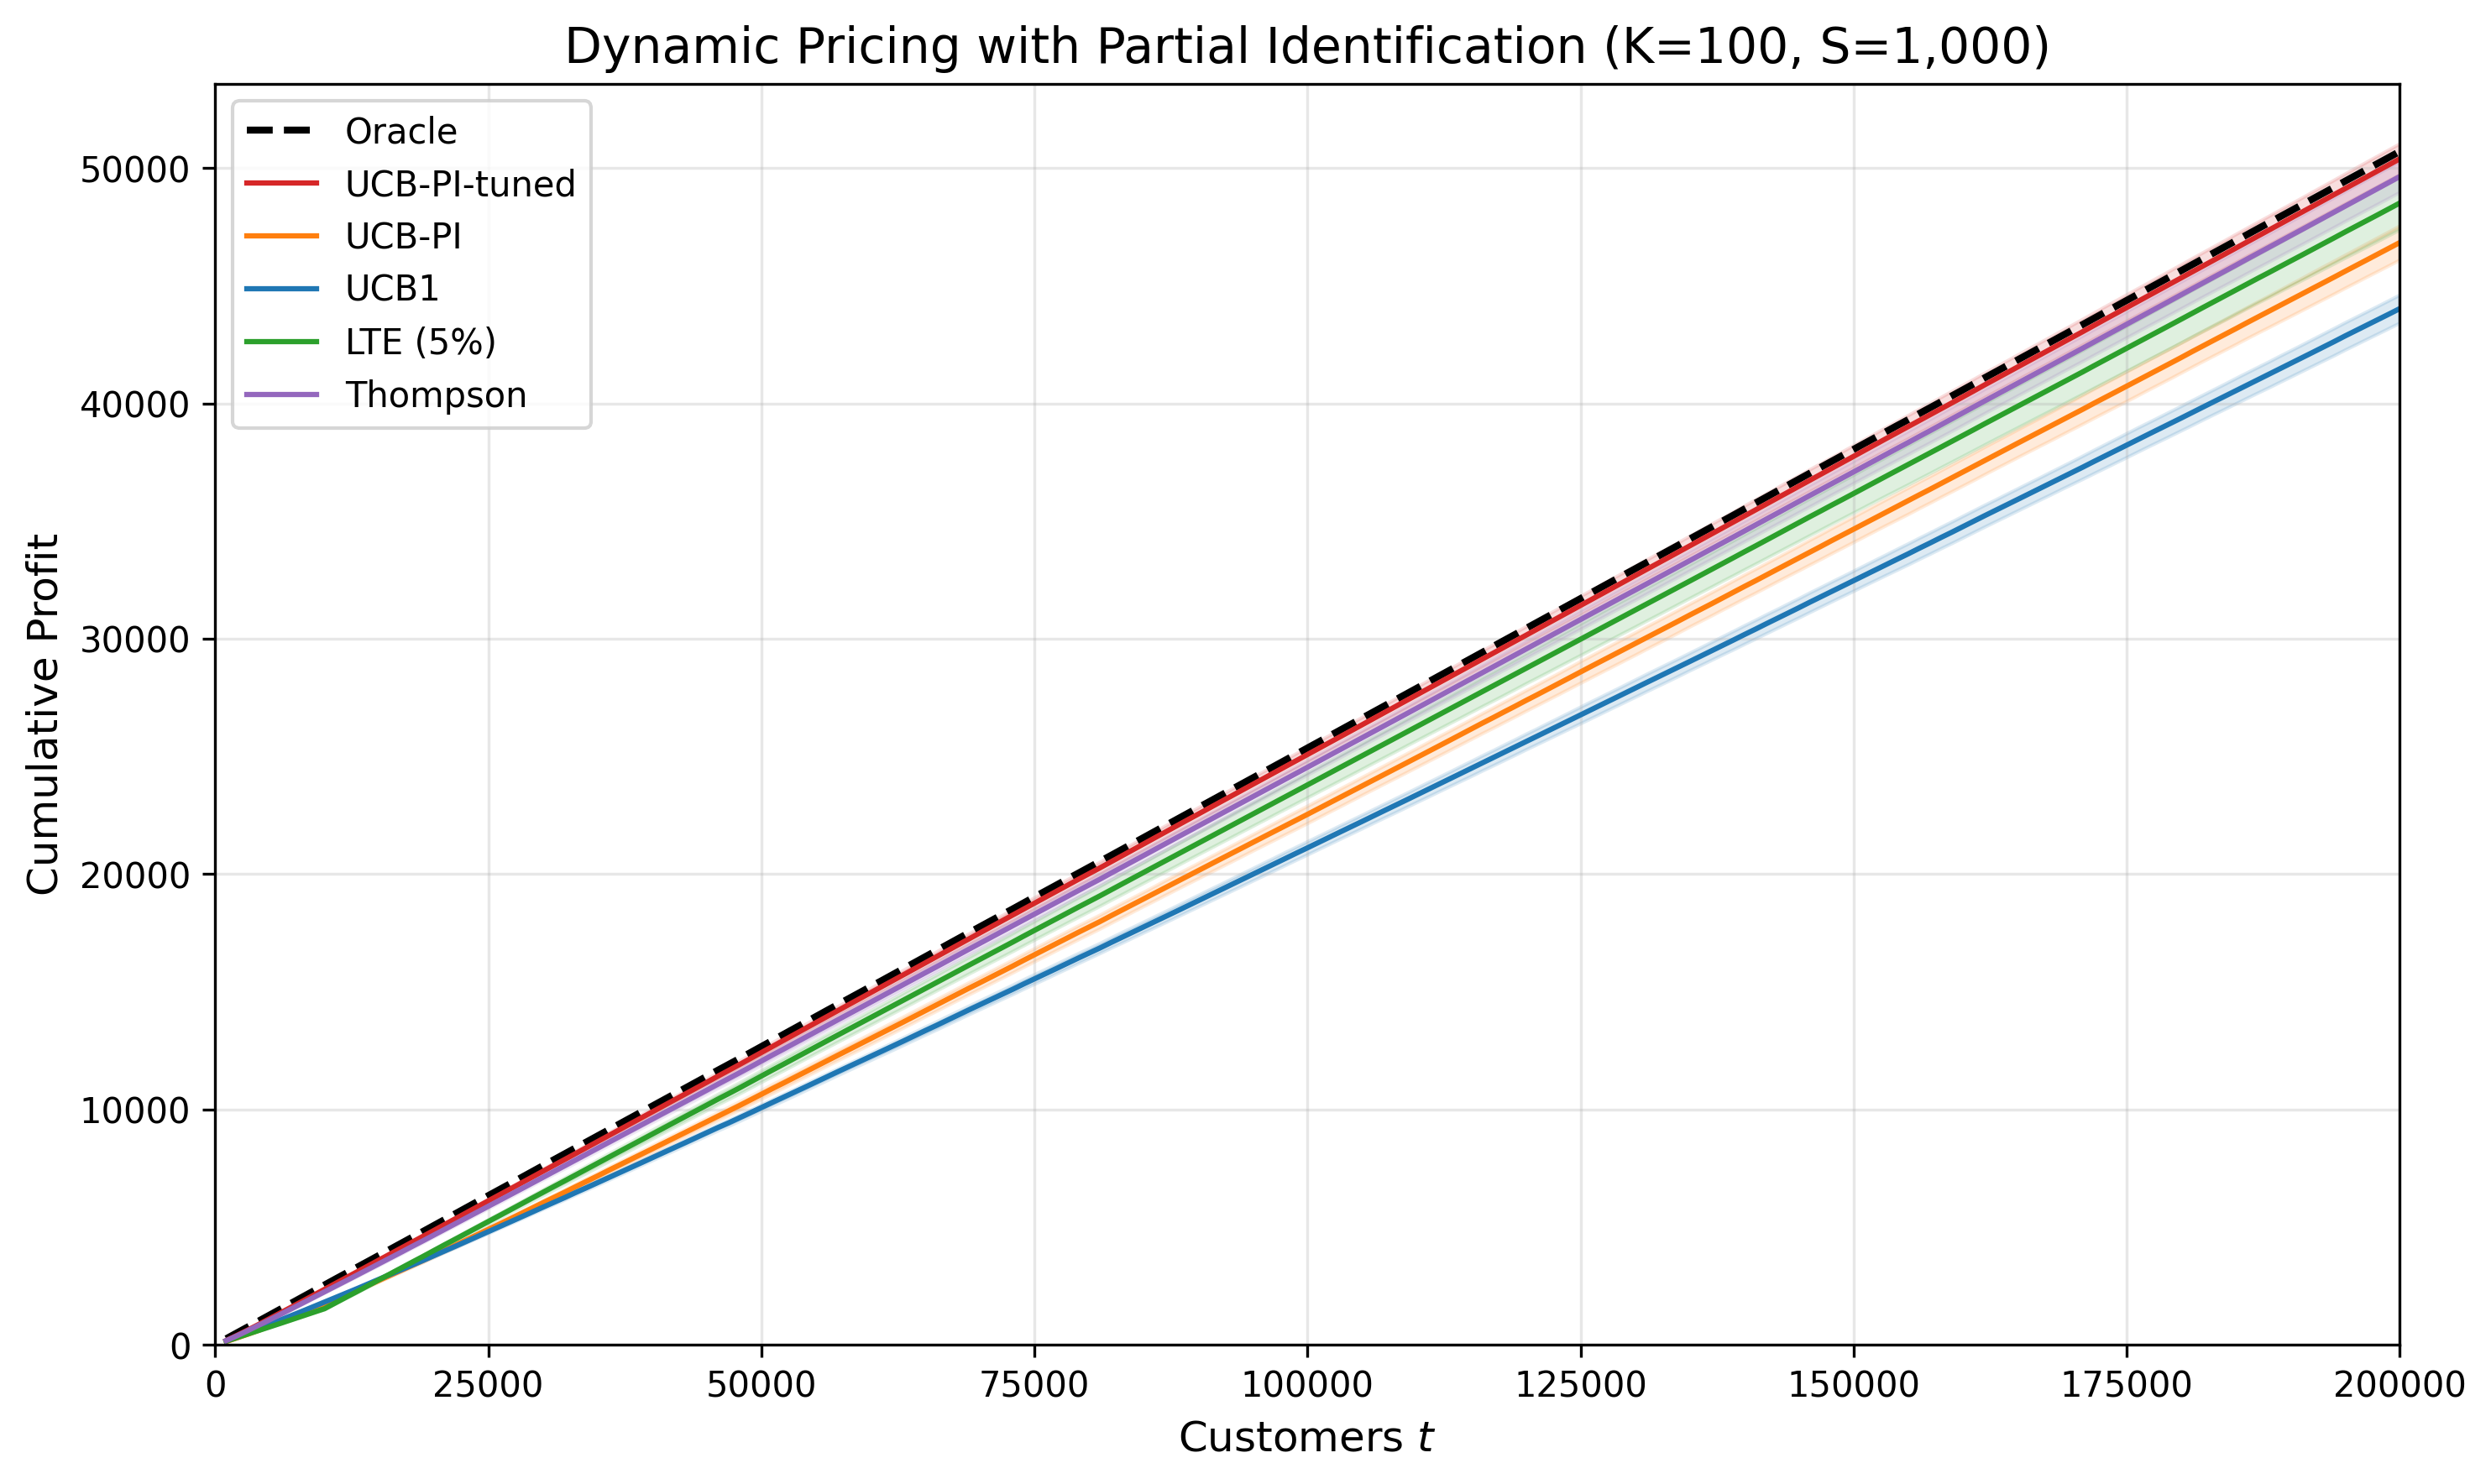
\includegraphics[width=0.9\textwidth]{../ch06_bandits/sims/structural_pricing_misra_profit.png}
\caption{Cumulative profit for dynamic pricing. Oracle (black) knows demand perfectly. Learning algorithms converge to near-optimal pricing. Shaded regions show $\pm 2$ standard errors.}
\label{fig:bandit_profit}
\end{figure}

The simulation validates two findings. First, the ``cost of learning'' is small: even without knowing the demand curve, UCB1 loses only 0.24\% of potential profit. Second, exploiting economic structure (unimodal revenue) enables efficient price search, though in this setting with moderate $K$, standard UCB performs comparably to the structure-aware OSUB. The advantage of unimodal algorithms grows with $K$.
